
\begin{quote}
"The single biggest problem in communication is the illusion that it has taken place" \\
\hspace*{\fill} — George Bernard Shaw 
\end{quote}

Now that we have more than a single protection domain, we need a way to communicate between them. In a traditional operating system, one can imagine wanting to be able to request that another process be killed so that a task manager might work, for example. This inter-process communication is even more fundamental to the operation of Barrelfish due to the lack of services in the kernel. When we spawn a new process, if that process wants RAM, it must ask for it from some other process that has capabilities to RAM already. In some sense, IPC is the glue that holds Barrelfish together. 

\subsubsection*{What We're Working With} \label{wwww}
Barrelfish comes with a library for transferring data and capabilities between dispatchers (that this is between dispatchers is important) already, in the form of Lightweight Message Passing. This library allows for non-blocking IPC by invoking a (retyped) capability to the other processes dispatcher, which pulls the kernel into the fray to work a little magic. On top of these raw endpoint capabilities, we have provided for us a channel abstraction, giving rise to "LMP Bindings" and the ability for a thread to wait for a message on such a channel.

Our goal with this milestone was to implement a fast and reliable framework for Remote Procedure Calls between protection domains, built on top of the LMP Channel abstraction. RPC aligns well with the kind of functionality we want out of this system: If a process wants more memory, we're fine with a synchronous call to request it. We also only need very small messages, since we can provide stubs for each of the functions. This means any single call can be made quite quickly. Given we'll be implementing printing to the terminal via this mechanism, our design has to minimize latency.

These operations are core to the function of Barrelfish, so we wanted them to be painless to use, easy to extend, fast, and most of all to seamlessly integrate with UMP (M6) when messages are passed across cores. We succeeded in some of these things.

\subsubsection*{A Messaging Layer Protocol} \label{msg_protocol}

To define a protocol, we need a conception of what a message looks like. The underlying LMP endpoints support transferring up to 8 words at a time, and channels give us a way of blocking and waiting on the dispatch/receipt of these packets. To enforce structure on two ends of a connection, one needs data that describes structure. If there's just one type of message, this can simply be globally agreed upon and fixed.  Given the number of possible RPC subroutines, we need some extra information to be sent with the message itself. We decided to sacrifice 1 word of payload space to pack in information about the length of the payload, its type (i.e. what sort of call we are making -- this lets us agree upon structure on each end), and some other information that is needed for handling messages larger than a single payload. With a message format in place, the task of both the client and server becomes marshalling and unmarshalling messages, and making their respective local function calls -- we have (semi) successfully decoupled our RPC from the underlying transport protocol.

\begin{lstlisting}[caption={RPC Structs}, label=lst:rpc_structs, language=C]
union rpc_hdr {
    struct {
        uint32_t pld_len;
        uint8_t type
        ...
    };
    uint64_t hdr_val;
};

struct rpc_msg {
    struct capref cap;
    union rpc_hdr hdr;
    uintptr_t pld[];
};
\end{lstlisting}

\subsubsection*{The Handshake} \label{handshake}

With an idea of \textit{what} we want to send in mind, we have to actually establish a connection. To keep the latency of each message low, Barrelfish borrows the concept of an explicit 'binding' from LRPC. That is, an LMP channel is persistent over the whole lifetime of a spawned process. Producing this binding is not a particularly interesting design choice, as there's a relatively fixed order. However, as a consequence of our choice to use \hyperref[sec:extending]{shared memory} to handle large messages, we introduce a small amount of complexity. Since all OS services live in the \verb|init| process (again, this is a design decision we made in light of time constraints), any spawned process must first share its endpoint capability to \verb|init| which in turn returns the capability to the shared memory buffer used to handle arbitrary sized messages. This exchange of capabilities is what constitutes our LMP handshake.

\begin{figure}[h!] 
	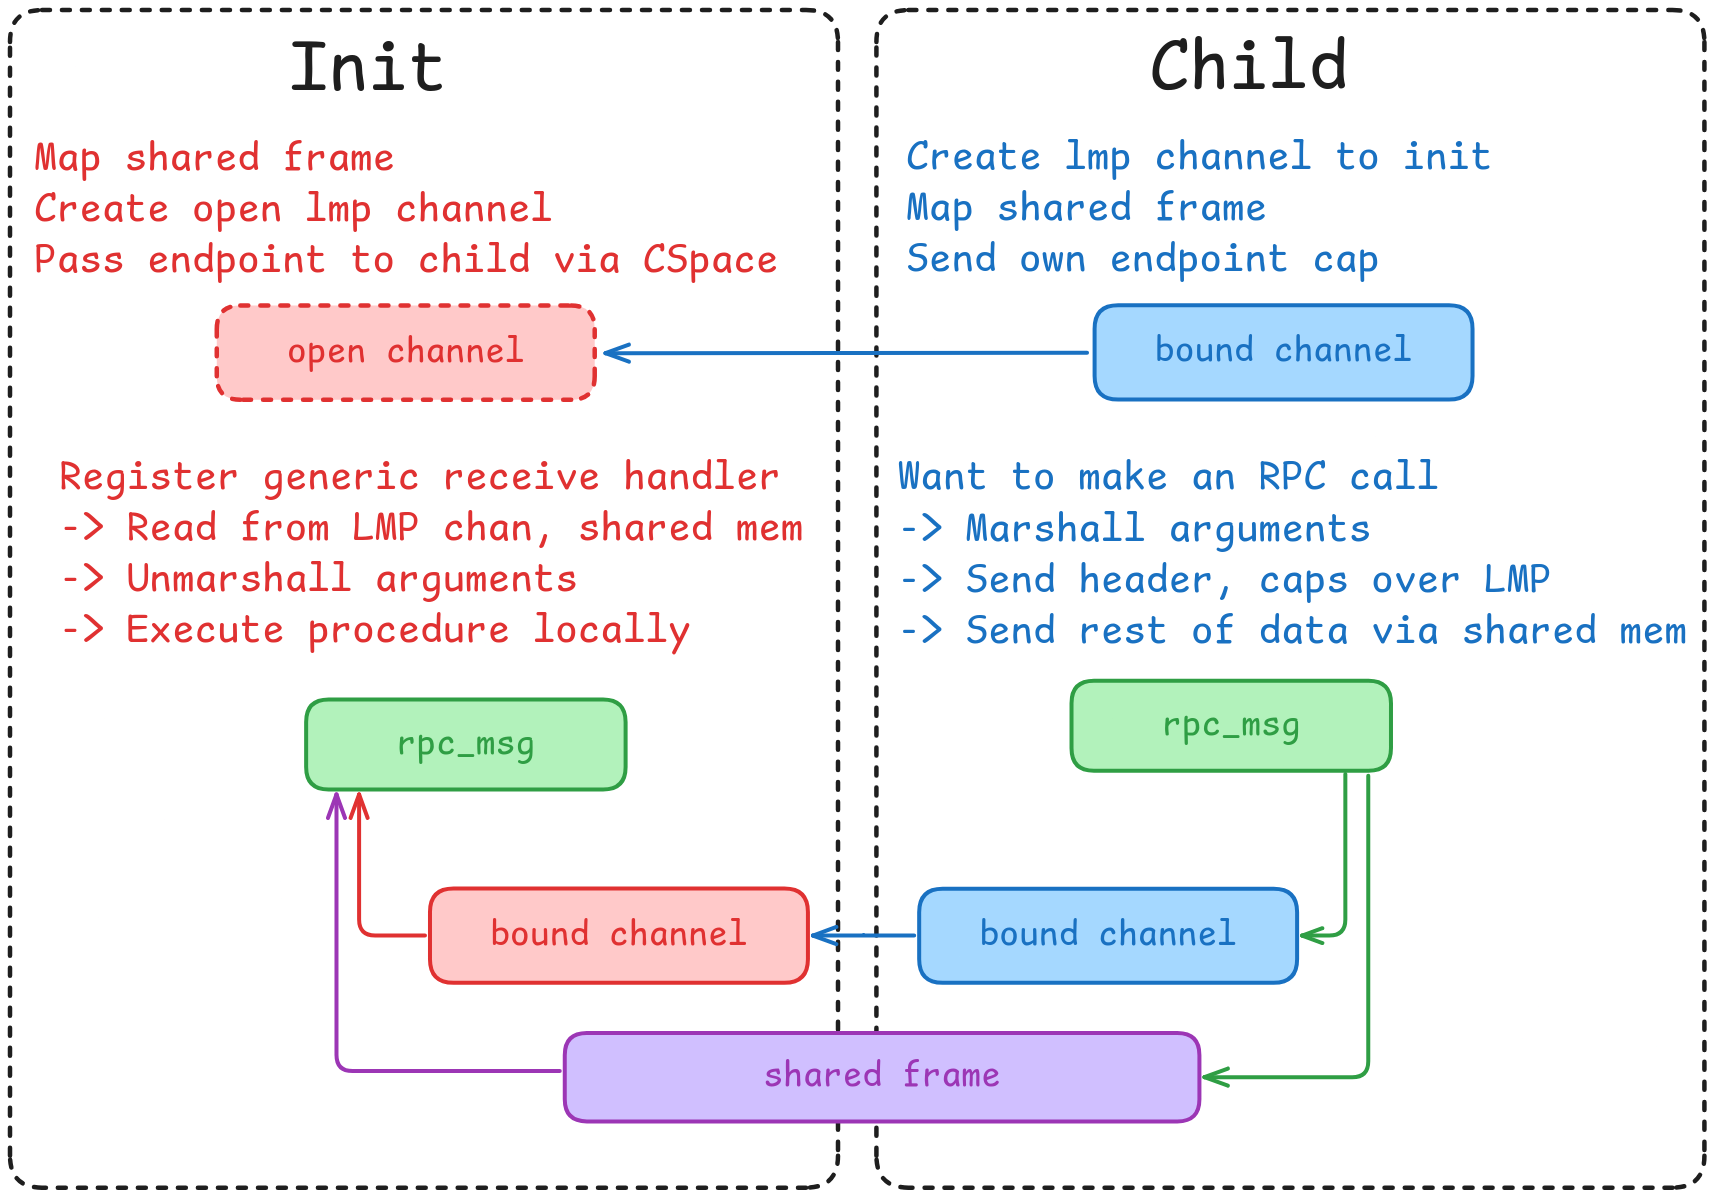
\includegraphics[width=\columnwidth]{report/images/handshake.png}
	\caption{The LMP Handshake}
	\label{figure:handshake}
	\centering
\end{figure}

\subsubsection*{The Big Picture} \label{sec:big_picture}

The final design of our message passing system can be seen in \autoref{figure:big_picture}. The \verb|burb| library sits at the core of this, handling marshalling/unmarshalling, dispatch logic and receiving messages. \verb|burb| is given an RPC message struct and returns an RPC message struct, hiding all of the underlying LMP logic away. Recall that our architecture stuffs all of the functionality of a memory server, terminal server, and process server into \verb|init|. On the server side then, \verb|burb| takes the form of a generic receive handler that is always registered, forwarding payloads to server-specific functions.

One key observation we made was that a given LMP channel is dispatcher to dispatcher, and hence the introduction of multiple threads on each process meant working with care. The simplest approach in this case was to enforce an invariant and make RPC send/receive pairs atomic. We have a mutex associated with each binding, and the thread making a call acquires the lock before sending a message, releasing it only after it has received a response. 

\subsubsection*{Flaws} \label{sec:flaws}

There are a number of flaws in this approach. The first and most obvious thing is that it severely limits the kinds of RPC calls we can make. Our invariant is that a call is always initiated by a client, and that this call may be treated as a single operation. This assumption was quickly violated when we considered implementing \verb|proc_mgmt_register_wait|, an RPC call that tells a thread to suspend until a specified process is killed. This call is \emph{open}, and with our current design, this could potentially intercept all other calls to the process hosting the suspended thread. We ended up not solving this issue. Perhaps more troubling was our assumption that the server would never want to send a message to a client without the client asking first. This immediately ruled out client-to-client communication via the server process and made a large chunk of M6 totally unviable.

It's worth noting that LMP channels are reliable, so we don't worry about messages failing to send. However, we have no time-out mechanism. If for whatever reason a thread is not able receive a message it expects, not only will it hang, but no further RPC calls will be able to be made by any thread on that process.

Lastly, as mentioned earlier, we decided to house all OS services in the \verb|init| process. This is less than ideal because this limits concurrent access to distinct services. It also means that if the \verb|init| process stops running, access to all services is lost. An ideal approach would have a process for each service along with a name server to enable service discovery.


\subsubsection*{Handling Large Messages} \label{sec:extending}

So what if we want to send messages larger than 7 words? There are a number of potential approaches. One choice is to simply split the message into many LMP messages, associate with each on a sequence number, and reconstruct the message on the other side of the channel. This is slow because we have to context switch for each message, and introduces plenty of opportunities for mistakes to be made in reconstructing the message. Another, arguably simpler approach, is to just share some memory between each process. In our design, we keep these messages synchronous and use LMP to transfer a header describing the message we've written to the shared memory frame. We support arbitrarily sized messages, but with an entire page of memory to work with, the vast majority of messages will only require a single read from this buffer. To illustrate the difference in performance, we have provided benchmarks in \autoref{figure:performance_lmp}, comparing shared memory to multiple LMP messages. This is cropped for readability. 
\begin{figure}[h!] 
	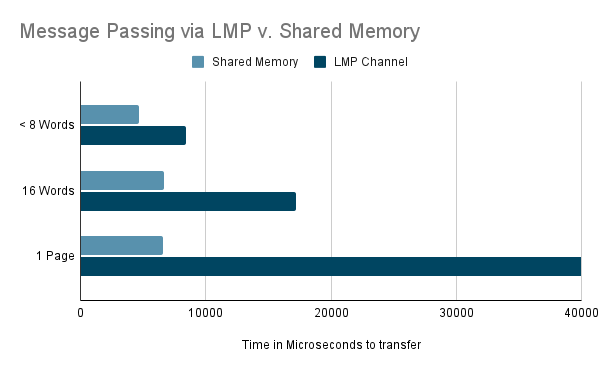
\includegraphics[width=\columnwidth]{report/images/Message Passing via LMP v. Shared Memory.png}
	\caption{Performance characteristics}
	\label{figure:performance_lmp}
	\centering
\end{figure}

And now without cropping (clearly, the number of context switches in the approach using raw LMP payloads dominate the time it takes to share 1 page worth of data and is multiple order of magnitudes slower than using a shared memory buffer).
\begin{figure}[h] 
	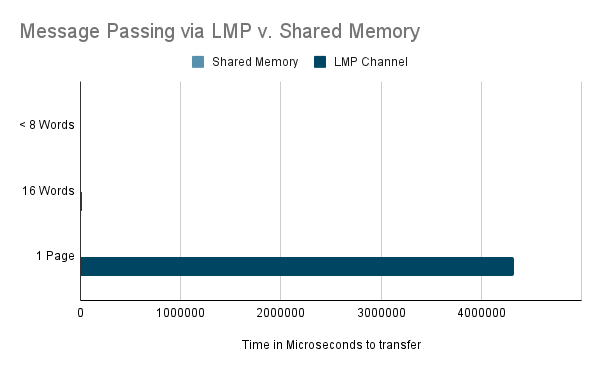
\includegraphics[width=\columnwidth]{report/images/Message Passing via LMP v. Shared Memory(1).png}
	\caption{Performance characteristics}
	\label{figure:performance_lmp_uncrop}
	\centering
\end{figure}

\begin{figure*}[h] 
	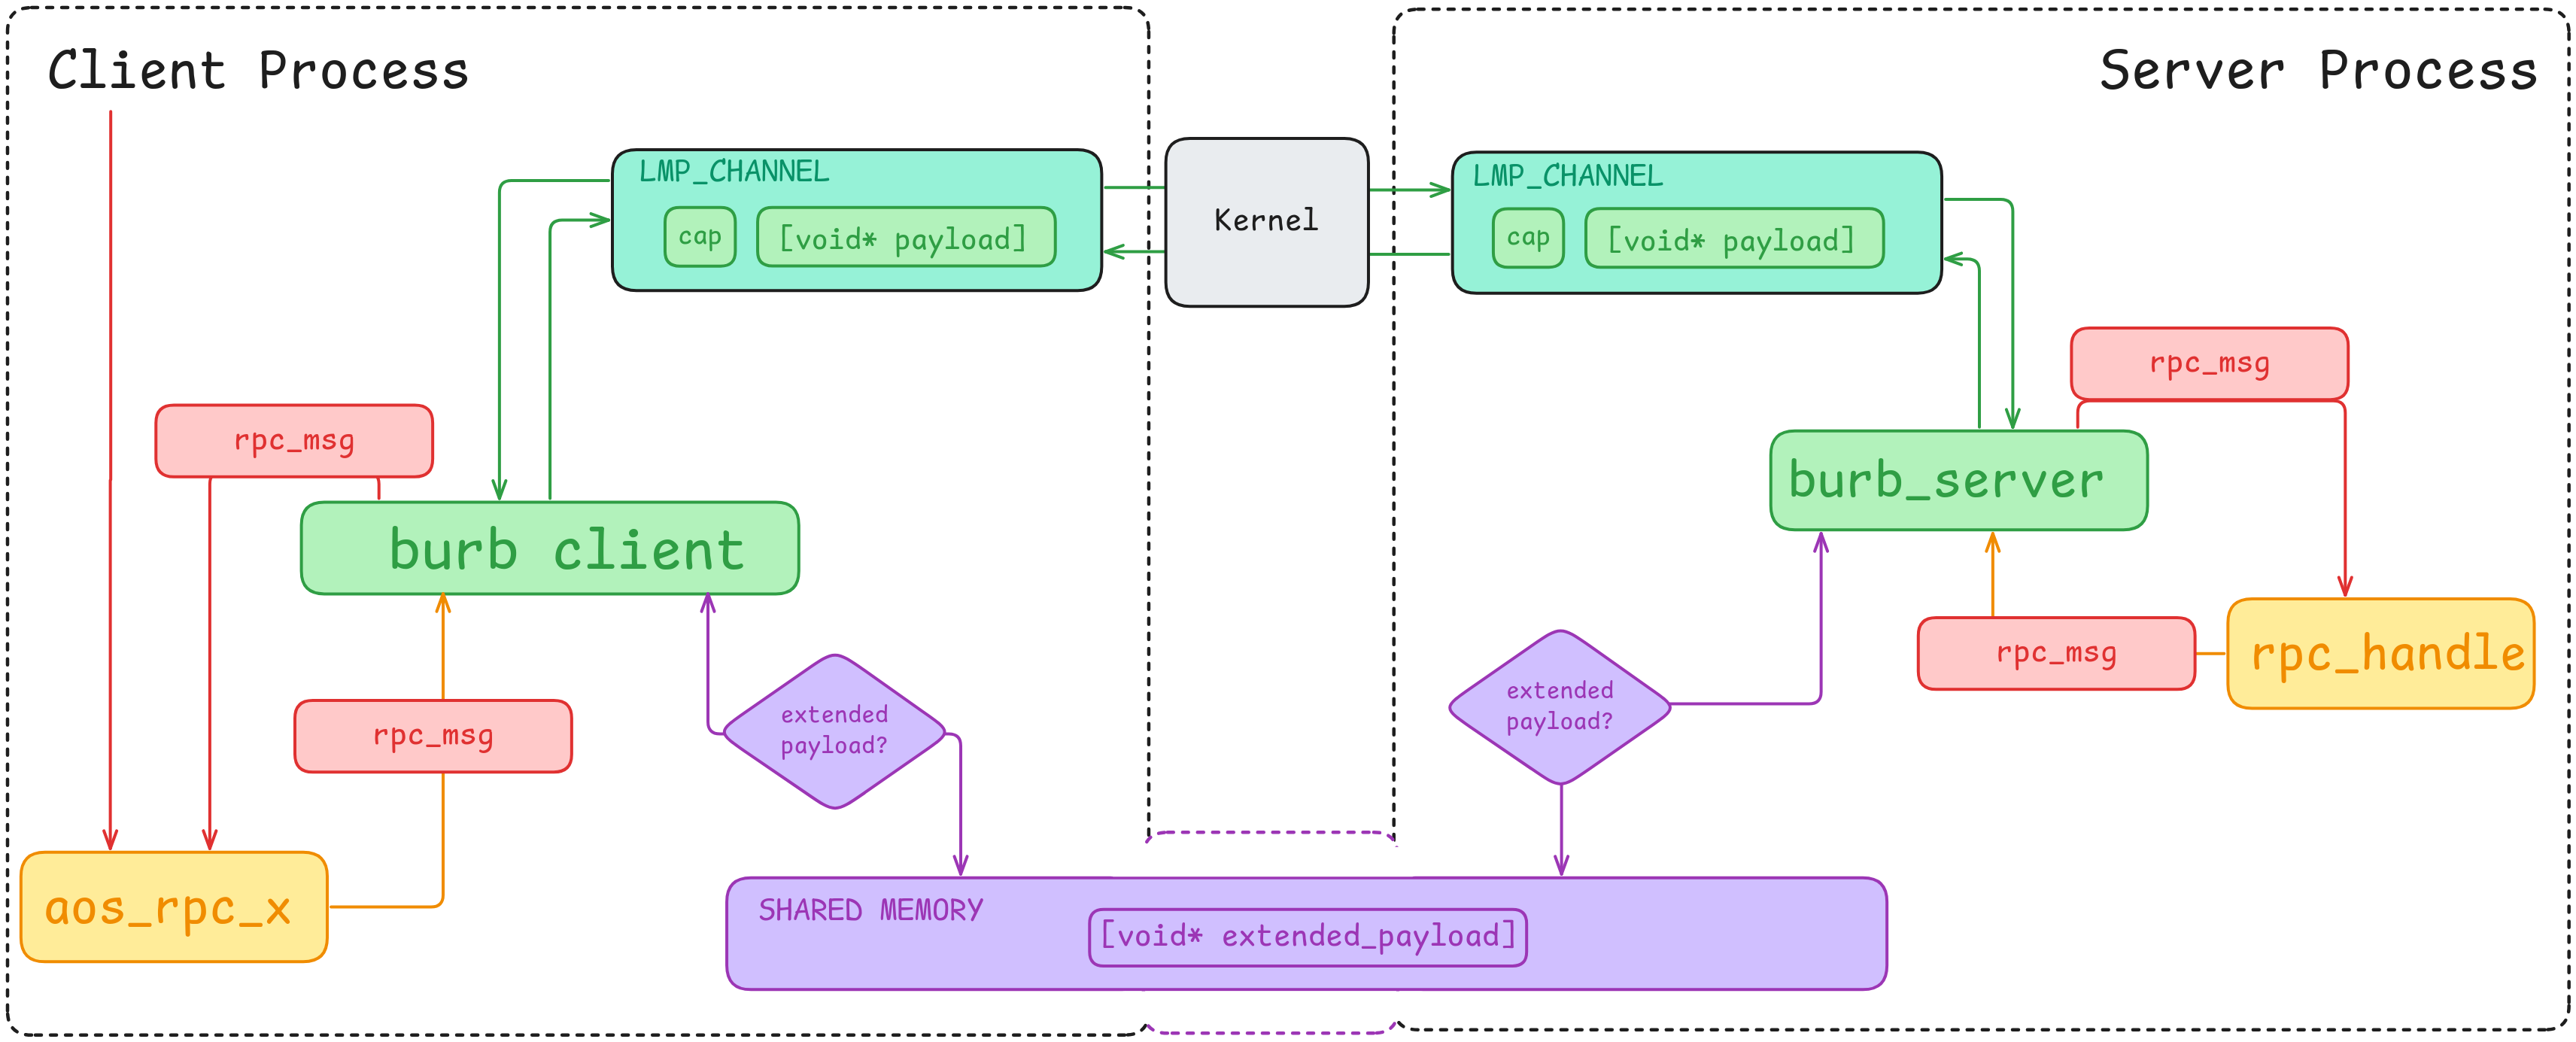
\includegraphics[width=\textwidth]{report/images/rpc_lmp.png}
	\caption{Our RPC System Design}
	\label{figure:big_picture}
	\centering
\end{figure*}
